\documentclass[conference]{IEEEtran}
\IEEEoverridecommandlockouts
% The preceding line is only needed to identify funding in the first footnote. If that is unneeded, please comment it out.
\usepackage{cite}
\usepackage{amsmath,amssymb,amsfonts}
\usepackage{graphicx}
\usepackage{textcomp}
\usepackage{xcolor}
\def\BibTeX{{\rm B\kern-.05em{\sc i\kern-.025em b}\kern-.08em
    T\kern-.1667em\lower.7ex\hbox{E}\kern-.125emX}}
\title{
\vspace{1cm}
{Assignment:
\\4-Bit Ring Counter on Arduino}
}
\author{Rajib Ghosh}
 \begin{document}
\maketitle
\section{ABSTRACT}
A ring counter is a special type of application of the Serial IN Serial OUT Shift register. The only difference between the shift register and the ring counter is that the last flip flop outcome is taken as the output in the shift register. But in the ring counter, this outcome is passed to the first flip flop as an input. All of the remaining things in the ring counter are the same as the shift register.

In this program, an LED was used for checking the output. The last flip-flop output was connected with the input of the initial flip-flop and Led bulb as well, to get the result.

\subsection{Truth Table for Ring Counter}
Truth Table for Ring Counter is given in Table: I
\begin{table}[htbp]
    \centering
\begin{tabular}{ | c | c | c | c | c | c | } \hline
ORI  & CLK & $Q_0$ & $Q_1$ & $Q_2$ & $Q_3$ \\\hline
low  & X   & 1 & 0 & 0 & 0 \\
High & Low & 0 & 1 & 0 & 0 \\
High & Low & 0 & 0 & 1 & 0 \\
High & Low & 0 & 0 & 0 & 1 \\
High & Low & 1 & 0 & 0 & 0 \\ \hline
\end{tabular}
\vspace{0.1cm}
\caption{\label{tab:widgets}}
\end{table}
\section{COMPONENTS}
Required components list given in Table: II.
\\Flip-flop IC 7474 diagram is shown in Figure 1.
\begin{figure}[h]
\centering
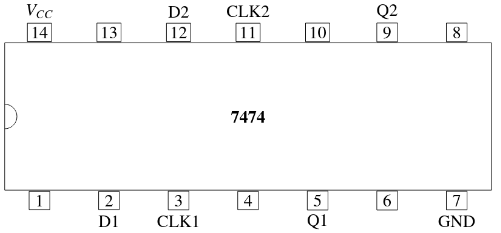
\includegraphics[width=0.4\textwidth]{7474.png}
\caption{\label{fig:Gates}}
\end{figure}
\begin{table}
\centering
\begin{tabular}{| c | c | c |} \hline
Components & Value & Quantity \\\hline
Resistors & 220 ohm & 1 \\
LEDs &  & 1 \\
Arduino & UNO & 1 \\
Jumper Wires &  & 20 \\
Breadboard & & 1 \\ 
\hline
\end{tabular}
\vspace{0.1cm}
\caption{\label{tab:widgets}}
\end{table}
\section{HARDWARE}
Make the connections between Arduino and LED as per the Table: III
\begin{table}
\begin{tabular}{|c | c | c | c | c | c | c |} \hline
 & \textbf{INPUT} & \textbf{INPUT} & \textbf{OUTPUT} & \textbf{OUTPUT} & \textbf{CLOCK} & \textbf{CLOCK} \\\hline
\textbf{7474} & 2 & 9 & 5 & 12 & CLK1 & CLK2 \\\hline
\textbf{7474} & 2 & 9 & 5 & 12 & CLK1 & CLK2 \\\hline 
\textbf{Arduino} & & & & & & 13 \\\hline
\textbf{LED} & LED1 &  &  &  & LED1 & \\\hline
\end{tabular}
\vspace{0.1cm}
\caption{\label{tab:widgets}}
\end{table}
\section{SOFTWARE}
Download the codes given in the link below and execute them.
https://github.com/rajib05ra/FWC-Assignments/tree/main/Assignment%20IDE/IDE%20Code%20run/src

\section{CONCLUSION}
A ring counter is a typical application of the Shift register. Here the output of the last flip-flop is connected to the input of the first flip-flop, which shift the register.After that, at each clock pulse, the preseted 1 is shifted to the next flip-flop and thus forms a Ring
\end{document}